\newcommand{\chapter}[2][]{
	\newcommand{\chapname}{#2}
	\begin{flushleft}
		\begin{minipage}[t]{\linewidth}
			
\includegraphics[height=1cm]{hdht-logo.png}
			\hspace{0pt}	
			\sffamily\bfseries\large Bài 3.
			\begin{flushleft}
				\Large\bfseries #1
			\end{flushleft}
		\end{minipage}
	\end{flushleft}
	\vspace{1cm}
	\normalfont\normalsize
}
\chapter[Giới thiệu ứng dụng của Vật lí trong một số ngành nghề:\\ Công nghiệp - Thông tin, dự báo thời tiết và nông nghiệp]{Giới thiệu ứng dụng của Vật lí trong một số ngành nghề:\\ Công nghiệp - Thông tin, dự báo thời tiết và nông nghiệp}
\section{Hình thành kiến thức mới}

\subsection{Hình thành kiến thức mới}
\subsubsection{Ứng dụng của Vật lí trong quân sự}
Theo sự tiến hóa của lịch sử, các ứng dụng của Vật lý trong quân sự cũng ngày càng tiến hóa hiện đại hơn

\begin{minipage}[l]{0.6\textwidth}
Ứng dụng nguyên lí hoạt động của các máy cơ đơn giản: cung tên, máy bắn đá,

Ứng dụng định luật bảo toàn động lượng, khí động lực học: súng trường, đại bác, súng hạng nặng, máy bay phản lực, máy bay tiêm kích, tên lửa phòng không,

Ứng dụng nguyên lí thu phát sóng điện từ: ra-đa, trinh sát, vệ tinh,

Ứng dụng nguyên lí Bernoulli, lực đẩy Archimedes: tàu ngầm, tàu sân bay,

Ứng dụng phản ứng hạt nhân: vũ khí hạt nhân,

Các ứng dụng khác: LASER, điện - điện tử, bán dẫn, vật liệu.
\end{minipage}
\begin{minipage}[r]{0.4\textwidth}
\begin{center}
	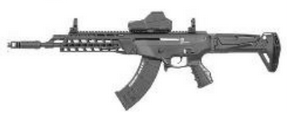
\includegraphics[scale=0.8]{../figs/G10-003-1.png}
\end{center}
\begin{center}
	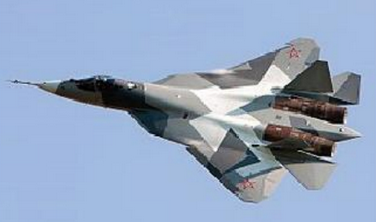
\includegraphics[scale=0.8]{../figs/G10-003-2.png}
\end{center}
\end{minipage}
\subsubsection{Ứng dụng của Vật lí trong công nghiệp hạt nhân}
Năng lượng hạt nhân hay năng lượng nguyên tử là một dạng năng lượng được giải phóng khi hạt nhân nguyên tử bị tách ra thành nhiều hạt nhân nhỏ hơn (phân hạch) hoặc các hạt nhân nhỏ hợp nhất thành hạt nhân lớn hơn (nhiệt hạch). Công nghệ hạt nhân được thiết kế để tách năng lượng hữu ích từ hạt nhân nguyên tử thông qua các lò phản ứng hạt nhân có kiểm soát.

Sử dụng năng lượng hạt nhân tới nay vẫn còn gây ra một số tranh cãi như: tạo ra chất thải nguy hại cho môi trường; quá trình vận hành có nguy cơ rủi ro và sự cố xảy ra khá cao. Tuy nhiên, cho đến nay, năng lượng hạt nhân vẫn được coi là một trong những nguồn năng lượng dồi dào góp phần đáp ứng nhu cầu năng lượng không ngừng tăng nhanh. Đồng thời, công nghệ hạt nhân còn được sử dụng rộng rãi trong các ngành nghề khác như y tế, công nghiệp, nông nghiệp, sinh học,...
\subsubsection{Ứng dụng của Vật lí trong khí tượng, thủy văn}
Khí tượng học nghiên cứu các hiện tượng và quá trình biến đổi của khí quyển và những hiệu ứng trực tiếp của khí quyển lên bề mặt Trái Đất, đại dương.

Thủy văn là ngành khoa học nghiên cứu về sự vận động, phân bố và chất lượng nguồn nước, bao gồm vòng tuần hoàn của nước và mối quan hệ của chúng với môi trường trong mỗi giai đoạn trong chu trình thủy văn.

Dựa vào thủy văn, con người có thể đưa ra các dự đoán ngắn - dài hạn nhằm phục vụ cho việc canh tác hoa màu, dự báo thiên tai. Tuy nhiên, các yếu tố liên quan đến khí tượng và thủy văn thường xuyên thay đổi theo thời gian và vị trí địa lí. Do đó, đòi hỏi con người phải xây dựng một ngành khoa học về thủy văn để thay thế cho kinh nghiệm quan sát thường ngày.

Việc dự báo thủy văn ngày càng trở nên quan trọng trong việc đảm bảo sự phát triển kinh tế xã hội và an ninh quốc gia bởi sự biến đổi khí hậu đang diễn ra vô cùng phức tạp trên phạm vi toàn cầu. Hiện nay, ngành khí tượng thủy văn đã xây dựng được một số mô hình vật lí - toán học cho dữ liệu lớn (big data), kết hợp với những siêu máy tính hiện đại để mô phỏng những diễn biến của thời tiết, thủy văn từ đó đưa ra những dự báo sớm và chính xác các sự kiện.

Nhân lực có chuyên môn về Vật lí chất lưu, Vật lí lí thuyết và tính toán sẽ có nhiều cơ hội việc làm tại các trung tâm dự báo khí tượng và thủy văn, các dự án quy hoạch.
\subsubsection{Ứng dụng của Vật lí trong nông, lâm nghiệp}
\begin{minipage}[l]{0.6\textwidth}
Vật lí học nông nghiệp nghiên cứu và ứng dụng những phương pháp, phương tiện nhằm điều chỉnh các điều kiện vật lí liên quan với đời sống cây trồng, chăn nuôi, nuôi trồng thủy sản, góp phần định hướng và phát triển một nền nông nghiệp an toàn và bền vững.

Bức xạ ion hóa gây đột biến và tạo ra các giống cây có đặc tính mới: tăng thẩm mỹ, tăng năng suất, đề kháng sâu bệnh, kích thích tăng trưởng,

Công nghệ nano được ứng dụng để tăng hiệu quả và an toàn của phân bón và thuốc bảo vệ thực vật làm tăng sản lượng và chất lượng cây trồng, hoặc phát hiện dư lượng thuốc trừ sâu và thuốc kháng sinh trong công tác kiểm định chất lượng sản phẩm.

Công nghệ kết nối không dây và thu phát sóng điện từ: kiểm tra chất lượng nguồn nước trên thiết bị di động, hệ thống tưới tiêu, thu hoạch, bón phân tự động, cảnh báo nguy cơ tiềm ẩn.

Bên cạnh đó, các máy móc hiện đại giúp tăng năng suất lao động, giảm các hoạt động con người trong môi trường độc hại cũng đóng vai trò quan trọng.
\end{minipage}
\begin{minipage}[r]{0.4\textwidth}
\begin{center}
	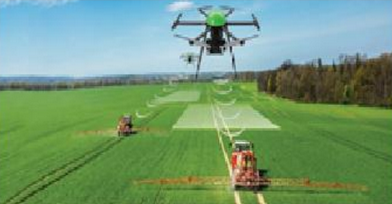
\includegraphics[scale=0.8]{../figs/G10-003-3.png}
\end{center}
\begin{center}
	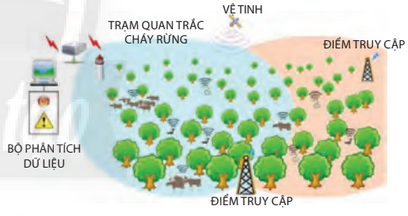
\includegraphics[scale=0.8]{../figs/G10-003-4.png}
\end{center}
\end{minipage}
\subsubsection{Ứng dụng của Vật lí trong điện tử}
\begin{minipage}[l]{0.6\textwidth}
Kĩ thuật điện tử nghiên cứu và sử dụng các thiết bị điện hoạt động theo sự điều khiển của dòng điện trong các thiết bị điện như đèn điện tử hay bán dẫn để thiết kế các mạch điện tử.

Các kiến thức về vật lí giúp nghiên cứu và chế tạo các linh kiện điện tử như LED, photodiode, diode laser, ... là các linh kiện chủ yếu trong các mạch điện tử để điều khiển, xử lí, chuyển đổi và phân phối nguồn điện, các ứng dụng này liên quan đến việc tạo ra và xác định trường điện từ và dòng điện.

Ngày nay, các linh kiện điện tử được tích hợp trên các mạch hay vi mạch tích hợp, hoặc mạch tổ hợp là tập hợp các mạch điện chứa các linh kiện bán dẫn, điện trở, ... được kết nối với nhau, để thực hiện một chức năng xác định. Các vi mạch này ngày càng được chế tạo với kích thước nhỏ hơn, mật độ transistor tăng lên giúp các thiết bị nhỏ gọn, tiêu tốn ít năng lượng và tăng hiệu suất xử lí.

Bên cạnh những đóng góp trong chế tạo vi mạch, ngành điện tử học còn nghiên cứu chế tạo và cải thiện hiệu suất của pin quang điện (pin mặt trời) để khai thác năng lượng sạch từ ánh sáng mặt trời.

Các kĩ sư hay nhà nghiên cứu về chất bán dẫn, chế tạo vi mạch, ... có nhiều cơ hội phát triển nghề nghiệp trong lĩnh vực điện tử.
\end{minipage}
\begin{minipage}[r]{0.4\textwidth}
\begin{center}
	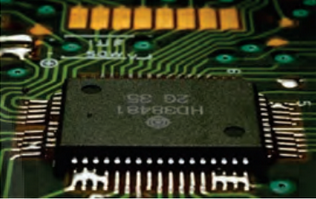
\includegraphics[scale=0.85]{../figs/G10-003-5.png}
\end{center}
\begin{center}
	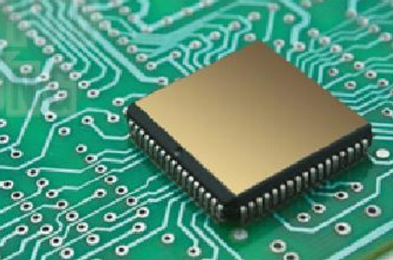
\includegraphics[scale=0.7]{../figs/G10-003-6.png}
\end{center}
\end{minipage}
\subsubsection{Ứng dụng của Vật lí trong cơ khí, tự động hóa}
Kĩ thuật cơ khí là một ngành kĩ thuật ứng dụng các nguyên lí vật lí, kĩ thuật và khoa học vật liệu để thiết kế, chế tạo và bảo dưỡng các loại máy móc và hệ thống cơ khí.

Linh vực kĩ thuật cơ khí cần sự am hiểu về cơ học, động lực học, nhiệt động lực học, khoa học vật liệu, năng lượng để thiết kế và chế tạo thiết bị công nghiệp và máy móc, ...

Công nghiệp tự động hóa sử dụng máy tính để kiểm soát, điều khiển máy móc thiết bị công nghệp và quy trình sản xuất, giảm bớt sự cần thiết phải can thiệp của con người.

Tự động hóa ngày càng có vai trò quan trọng trong đời sống, ngày càng có nhiều thiết bị tự động hóa kết hợp với trí tuệ nhân tạo để tạo ra các hệ thống thông minh.	 Các dây chuyền sản xuất tự động hóa và máy móc cơ khí chính xác cao trong các nhà máy đều cần nhân lực am hiểu về Vật lí để điều khiển. Ngoài ra, các công ty công nghệ luôn cần nguồn nhân lực chất lượng cao để phát triển những công nghệ mới.
\subsubsection{Ứng dụng của Vật lí trong thông tin, truyền thông}
Ngày nay, thế giới trở nên "phẳng" hơn trong thông tin liên lạc nhờ vào hệ thống internet và các thiết bị công nghệ như máy tính cá nhân, điện thoại thông minh, ...

Việc phát triển các công nghệ máy tính, điện thoại thông minh là một sự kết hợp giữa rất nhiều ngành khoa học, trong đó Vật lí nghiên cứu những nền tảng ban đầu.

Phương pháp nghiên cứu của vật lí thâm nhập vào nhiều lĩnh vực như quang học, vật lí chất rắn, ... 

Linh vực phát triển nhanh nhất của viễn thông là truyền dữ liệu. Mạng truyền dữ liệu là mạng thông tin được tạo thành bằng cách nối các nguồn tin với nhau, tiêu biểu là thông tin trên mạng internet. Trong tương lai gần, các công nghệ mạng không dây sẽ đóng vai trò quan trọng trong công nghệ định vị, dẫn đường, internet vạn vật (IoT), ... và mở ra thời kì chuyển đổi số mạnh mẽ.

Các kĩ sư, nhà vật lí sẽ có nhiều cơ hội việc làm không chỉ tại các cơ sở nghiên cứu mà còn ở các công ty công nghệ và truyền thông để phát triển các phương pháp truyền thông mới, hiệu quả và bảo mật hơn với công nghệ lượng tử.
\subsection{Mở rộng}
\subsubsection{Từ xu hướng tích hợp môn học đến xu hướng liên ngành}
Dạy học tích hợp là định hướng dạy học giúp học sinh phát triển khả năng huy động tổng hợp kiến thức, kĩ năng, ... thuộc nhiều lĩnh vực khác nhau để giải quyết các vấn đề trong học tập và trong cuộc sống. Xu hướng này diễn ra vì các lí do sau:
\begin{itemize}
	\item Đổi mới giáo dục tập trung phát triển phẩm chất và năng lực người học: giúp việc học tập gắn liền với thực tiễn hơn thông qua việc phát triển các phẩm chất và năng lực cần thiết;
	\item Mỗi sự vật, hiện tượng đều là thể thống nhất và có mối liên hệ với các sự vật, hiện tượng khác. Vì vậy, để nhận biết hoặc giải quyết mỗi sự vật, hiện tượng đều cần huy động tổng hợp kiến thức và kĩ năng từ nhiều lĩnh vực khác nhau;
	\item Khi tích hợp liên môn học, các kiến thức liên quan với nhau sẽ được lồng ghép vào cùng một môn học nên tránh được sự trùng lặp kiến thức, từ đó số lượng môn học và thời lượng học tập được giảm bớt;
	\item Do thực tiễn luôn thay đổi, nên việc trang bị phẩm chất và năng lực cốt lõi giúp cho người học thích nghi tốt hơn với những biến động và thách thức. Xu hướng tích hợp liên môn có tác dụng tích cực trong yêu cầu này.
\end{itemize}

	Giáo dục Việt Nam lâu nay chú trọng vào đào tạo chuyên ngành, thế nhưng, nhu cầu cho thị trường lao động mới cần nhiều hơn kiến thức chuyên ngành đơn lẻ. Người học cần được trang bị kiến thức đa ngành, tổng hợp để có một cách nhìn tổng quan, đáp ứng yêu cầu của nhà tuyển dụng trong bối cảnh mới.
	
	Xu hướng liên ngành không chỉ là sự kết hợp giữa các ngành riêng lẻ lại với nhau, mà còn có sự giao thoa giữa chúng để tạo ra các phẩm chất và năng lực mới. Đào tạo liên ngành trang bị cho người học những giá trị cốt lõi và đang trở thành một xu hướng tất yếu trong quá trình nhận thức của con người.
\subsubsection{Công dân toàn cầu}
Công dân toàn cầu (Global citizen) là khái niệm chỉ những người có thể sinh sống, làm việc và học tập mà không gặp các vấn đề về rào cản ngôn ngữ, biên giới, văn hóa, chính trị, ...  Họ được xem như là những người "Study anywhere - Live anywhere - Work anywhere".

Ở Việt Nam, xu hướng đào tạo công dân toàn cầu đã được triển khai ngay từ bậc mẫu giáo ở một số cơ sở đào tạo quốc tế, và phổ biến hơn ở bậc Đại học.

Người có tố chất của công dân toàn cầu thường có việc làm tốt và thu nhập trung bình cao. Bên cạnh đó, họ còn có đời sống tinh thần phong phú nhờ các trải nghiệm đa dạng. Đặc biệt, tố chất của một công dân toàn cầu đã được chứng minh là có thể xây dựng được thông qua nỗ lực làm việc và học tập của từng cá nhân.

Các tiêu chí của một công dân toàn cầu bao gồm:
\begin{itemize}
	\item Global knowledge - Kiến thức toàn cầu: Công dân toàn cầu có xu hướng quan tâm đến các vấn đề mà cả thế giới đang quan tâm, họ liên tục chủ động cập nhật kiến thức mới và coi việc học là quá trình diễn ra suốt đời.
	\item Global skills - Kĩ năng toàn cầu: Công dân toàn cầu quan tâm về những kĩ năng mà có thể giúp họ ứng dụng được kiến thức đã học vào môi trường thực tế , đặc biệt là kĩ năng về ngoại ngữ, tin học, kĩ năng phản biện và giải quyết vấn đề, kĩ năng làm việc nhóm, giao tiếp, kĩ năng nhận diện cảm xúc và phát triển trí tuệ cảm xúc, ...
	\item Global employment - Việc làm toàn cầu: Với kĩ năng, kiến thức toàn cầu, những người công dân toàn cầu có khả năng làm việc trên toàn thế giới. Do lợi ích của toàn cầu hóa và cách mạng công nghiệp 4.0 mang lại, cơ hội việc làm toàn cầu đang trở nên phong phú và đa dạng hơn bao giờ hết.
\end{itemize}
\section{Mục tiêu bài học - Ví dụ minh họa}
\begin{dang}{Mô tả được ví dụ thực tế về việc sử dụng kiến thức vật lí trong một số lĩnh vực}
	\viduii{3}{Hãy tìm hiểu trên internet về những nghiên cứu đột phá của vật lí nhằm thúc đẩy sự hình thành và phát triển của các loại vũ khí quân sự hiện đại.
	}
	{	\begin{center}
			\textbf{Hướng dẫn trả lời}
		\end{center}
		
		Học sinh có thể tìm hiểu về các loại vũ khí quân sự hiện đại ứng dụng dựa trên vật lí theo các từ khóa sau:
		\begin{itemize}
			\item Tên lửa dẫn đường;
			\item Sonar;
			\item Rađa;
			\item Bom hạt nhân;
			\item Tàu ngầm hạt nhân;
			\item Bom nhiệt hạch.
		\end{itemize}
	}
	\viduii{3}{Hãy tìm hiểu về cách hoạt động của một hệ thống thông minh cụ thể: nhà thông minh, nông nghiệp thông minh, thành phố thông minh.
	}
	{	\begin{center}
			\textbf{Hướng dẫn trả lời}
		\end{center}
		
		Học sinh tìm hiểu về các lĩnh vực cụ thể trong thiết kế hệ thống thông minh, với các tiêu chí sau:
		\begin{itemize}
			\item Giới thiệu về hệ thống;
			\item Đặc tính chung của hệ thống;
			\item Các thành phần trong hệ thống;
			\item Phân tích dữ liệu thu thập được từ hệ thống;
			\item Mạng cảm biến dùng trong hệ thống.
		\end{itemize}
		
	}

	\viduii{3}{Tìm hiểu về sự hình thành và phát triển của mạng internet từ lúc đầu cho đến khi xuất hiện hệ thống mạng toàn cầu (World Wide Web).
	}
	{	\begin{center}
			\textbf{Hướng dẫn trả lời}
		\end{center}
		
		Học sinh tìm hiểu về tiền thân của mạng Internet, sự xuất hiện của thuật ngữ Internet và các mốc lịch sử quan trọng trong quá trình phát triển Internet cho đến khi trở thành mạng toàn cầu.
		
	}
	\viduii{3}{Tìm hiểu về phương pháp chiếu xạ có tác động lên sự sinh trưởng của hạt giống và cho một số ví dụ cụ thể.
	}
	{	\begin{center}
			\textbf{Hướng dẫn trả lời}
		\end{center}
		
		Một số ví dụ cụ thể có thể kể đến gồm:
		\begin{itemize}
			\item Chiếu xạ tạo ra lan đột biến;
			\item Chiếu xạ tạo cam sành không hạt;
			\item Dùng công nghệ đột biến phóng xạ gamma tạo ra giống lúa có khả năng kháng sâu bệnh và tăng giới hạn chịu đựng, tăng năng suất.
		\end{itemize}
	}
\end{dang}